% Generator: hand-authored TikZ schematic traced from the fixed source; preserve the printed vertex labels verbatim.
% Source ID: src-dcc6a2c21c7b8e7b8f23f5188f34d7f542f94e40f4219b54cfb85a0d7004bc0f
% PDF SHA-256: 7fc0fd289fc486a0ae1c16a9ab5b4f0561830897df6e8897c50666f03d511913
% PDF page 2; printed page 127; question 18.
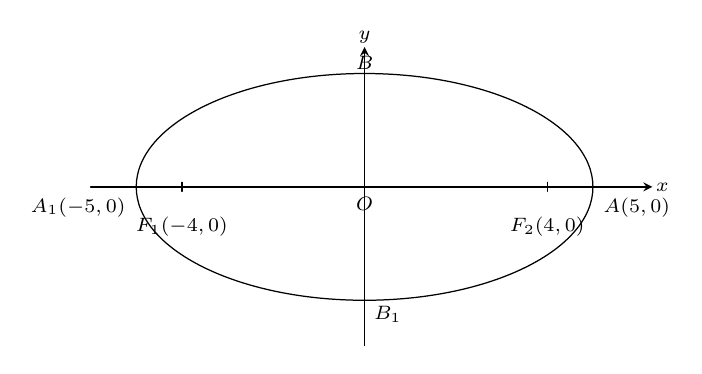
\begin{tikzpicture}[
  x=0.58cm,y=0.48cm,line width=0.45pt,line cap=round,>=stealth,
  every node/.style={font=\scriptsize,inner sep=1.2pt}
]
  \draw[->] (-6.0,0)--(6.3,0) node[right] {$x$};
  \draw[->] (0,-4.2)--(0,3.7) node[above] {$y$};
  \draw (0,0) ellipse [x radius=5,y radius=3];
  \draw (-4,-0.12)--(-4,0.12) (4,-0.12)--(4,0.12);

  % Coordinate labels match the source figure, including its A/A_2 inconsistency.
  \node[below left] at (-5.15,-0.18) {$A_1(-5,0)$};
  \node[below] at (-4,-0.7) {$F_1(-4,0)$};
  \node[below] at (0,-0.18) {$O$};
  \node[below] at (4,-0.7) {$F_2(4,0)$};
  \node[below right] at (5.15,-0.18) {$A(5,0)$};
  \node[above] at (0,3) {$B$};
  \node[below right] at (0.12,-3.05) {$B_1$};
\end{tikzpicture}
